\documentclass[../Dissertation.tex]{subfiles}

\begin{document}

\subsection{Overview}
\emph{
\begin{itemize}
	\item Questions to be addressed
	\item Metrics to be measured - why
\end{itemize}
}

This section will discusss the methodology used to search for lower latency models by tweaking pruning parameters.

%! ---------------------------------------------------------------------------------------------------------------------------------
\subsection{Conceptual Process}
\emph{
\begin{itemize}
	\item Sensitivity analysis - filter/channel selection and layer interdependencies
	\item Filter pruning implementation - Theory
	\item Channel pruning implementation - Theory
	\item Retraining pruned model
\end{itemize}
}
 

%! ---------------------------------------------------------------------------------------------------------------------------------
\subsection{Filter and channel selection}
\emph{
Link back to selected model - concrete examples of process described in previous section
\begin{itemize}
	\item Filter selection (visual representation of filters)
	\item Channel selection (visual representation of channels)
	\item Discussion of pruning consequences (and recovery) -> top1/top5 before retraining and after
\end{itemize}
}
%! ---------------------------------------------------------------------------------------------------------------------------------
\subsection{Engineering/implementation details}
\emph{
\begin{itemize}
	\item High level overview of physical system - justify need for multiple training agents
    \item Pruning \& retraining setup - Distiller (Pruning \& training)
	\item Benchmarking setup - openvino + benchmark (getting latency/throughput)
	\item Data processing - wandb + data visualisation steps
\end{itemize}
}

\newpage
%! ---------------------------------------------------------------------------------------------------------------------------------
\subsubsection{High level overview of system}

Figure~\ref{fig:agentCommunication} shows how each system interacts in the workflow, pruning is handled by the agent/s marked `Producer', benchmarking is handled by the `Consumer' agent, and the wandb system serves the next set of sweep parameters to each of the `Producer' agents.

\begin{figure}[H]
    \centering
    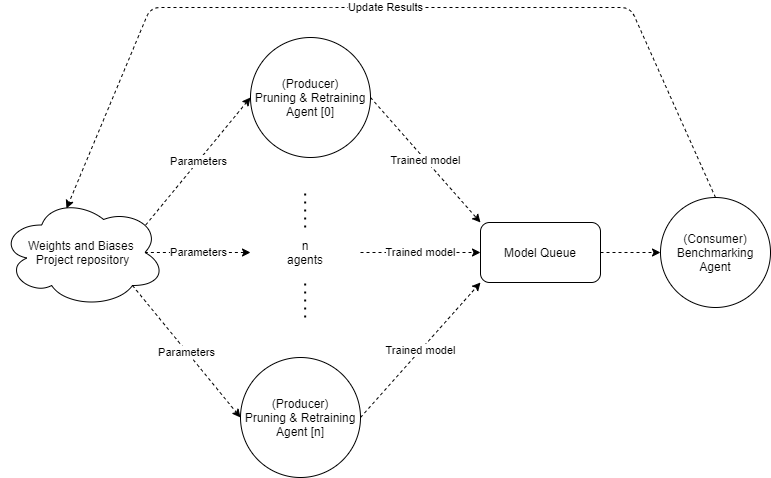
\includegraphics[width=\textwidth]{./ProducerConsumer}
    \caption{Diagram showing agent communication}
    \label{fig:agentCommunication}
\end{figure}

When pruning begins, the producer agent requests the (initially random) pruning parameters from the Weights and Biases Project server, the producer then applies the pruning algorithm and begins retraining the model.
Upon completion of retraining the model is exported into ONNX format and added to a queue for the consumer (the benchmarking agent) to benchmark and record the results, these results are then logged to weights and biases.
As described in \textbf{(TBD)} the parameter importance and correlation with the target metric is re-computed each time results are logged this can help determine in what direction to tune the paramater settings to minimise (or maximise) the target metric.

The runtime of a full benchmark for one model on the NCS is usually at most 5 seconds, pruning and retraining the network however can take between 20 - 120 mins depending on the network size and number of epochs. 
To imporve the efficiency of the training we separated the benchmarking system (consumer) from the pruning and retraining systems (producer), this made it easy to add new pruning and benchmarking agents to a single experiment or run multiple experiments in parallel.

%! ---------------------------------------------------------------------------------------------------------------------------------
\subsubsection{Defining parameters to prune}

\singlespacing
\begin{figure}[H]
    \begin{minted}[breaklines]{yaml}
        pruners: 
            layer_1_conv_pruner:
                class: 'L1RankedStructureParameterPruner'
                group_type: Filters
                desired_sparsity: 0.9
                weights: [
                    module.layer1.0.conv1.weight,
                    module.layer1.1.conv1.weight
                ]
        lr_schedulers:
            exp_finetuning_lr:
                class: ExponentialLR
            gamma: 0.95

        policies:
            - pruner:
                instance_name: layer_1_conv_pruner
                epochs: [0]
            
            - lr_scheduler:
                    instance_name: exp_finetuning_lr
                starting_epoch: 10
                ending_epoch: 300
                frequency: 1
    \end{minted}
    \caption{Example distiller schedule file, showing the pruning algorithm selected, and that algorithms parameters}
    \label{fig:CompressionSchedule}
\end{figure}
\doublespacing

Figure~\ref{fig:CompressionSchedule} shows a example compression schedule document in .yaml format which will provide instructions to Distiller to use the `L1RankedStructureParameterPruner' algorithm (section \textbf{TBD}) to prune the weights in each of the convolutions visible inside the `weights' array, specifying filter pruning and a target sparsity.

The pruning schedule is composed of lists of sections that define Pruners, LR-schedulers, and policies. A Pruner defines a pruning algorithm and the layers on which that pruning algorithm will be applied, LR-schedulers define the \textbf{learning-rate decay(Definition required)} algorithm. 
Finally each policy references the instance of the pruner or LR-scheduler it is managing (instance\_name), and controls when the respective algorithm will be applied, such as the start and end epoch, and the frequency of application.

\begin{figure}[H]
    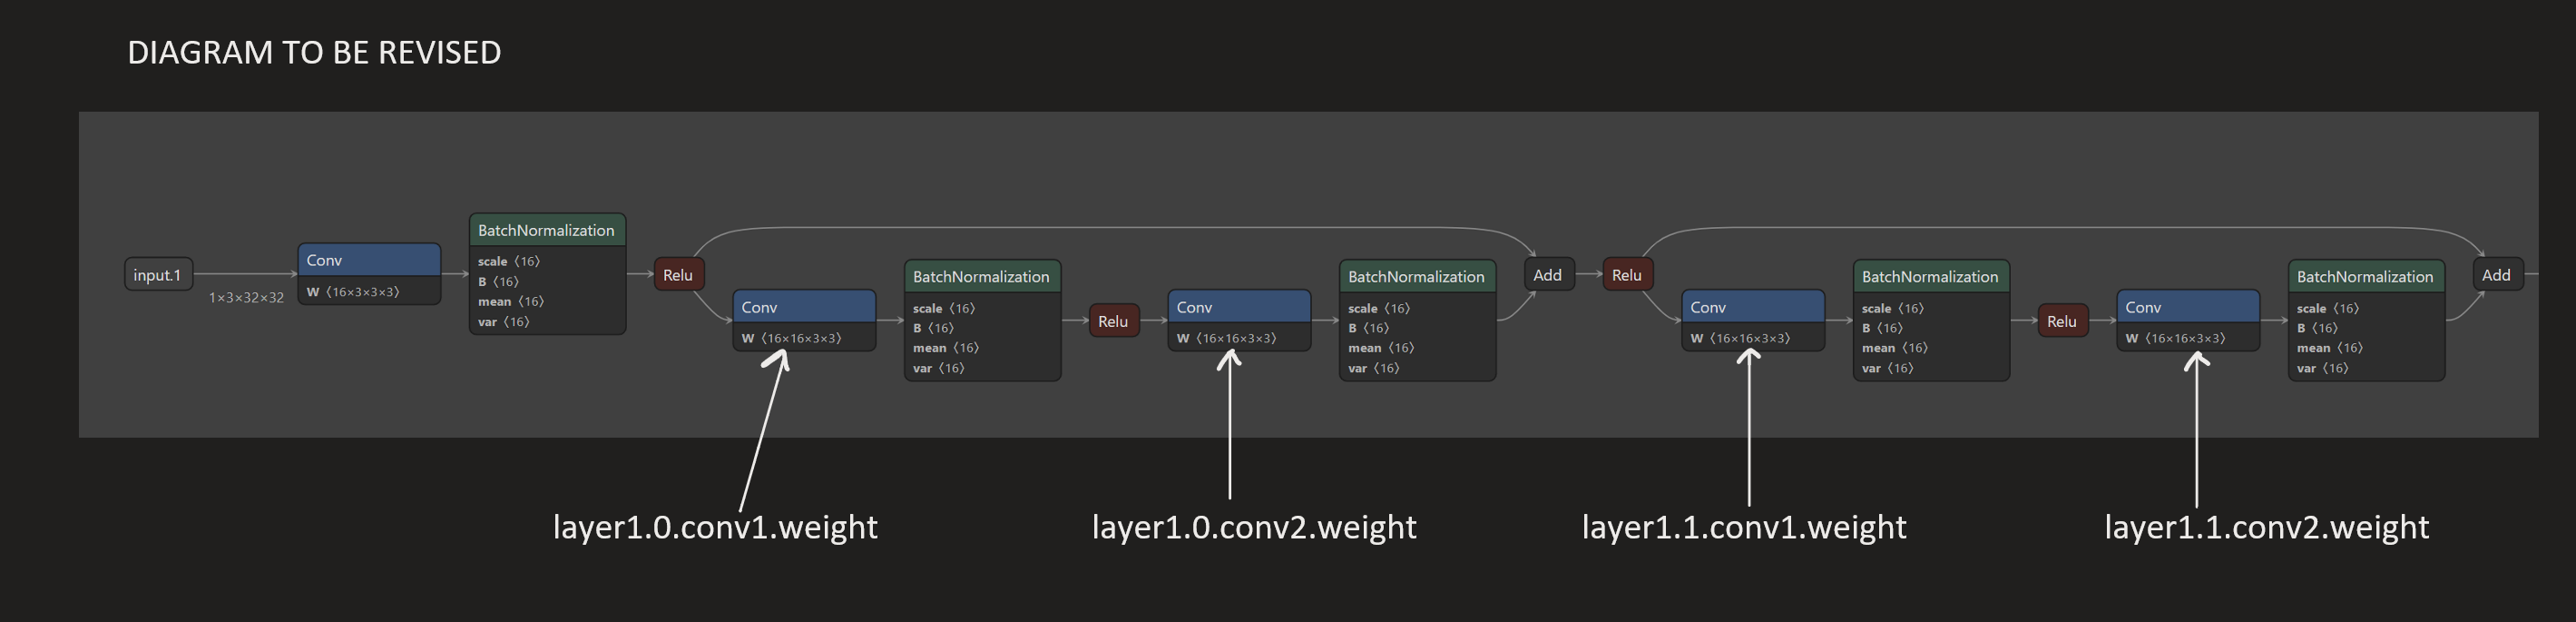
\includegraphics[width=\textwidth]{temp_pruning_layers.png}
    \caption{Resnet56 example showing wieght labels. \textbf{(TODO: rescale and redraw to highlight pertinent information)}}
    \label{fig:resnet56weightlabels}
\end{figure}

Each layer in the network is labelled either manually or automatically (see figure~\ref{fig:resnet56weightlabels}), distiller uses these labels to identify which layers being referenced by the compression schedule. 



%! ---------------------------------------------------------------------------------------------------------------------------------
\subsubsection{WandB API}

\begin{table}[H]
    \begin{tabular}{@{}|l|l|l|@{}}
    \toprule
    Key        & Description                    & Value                                    \\ \midrule
    program    & Script to be run               & Path to script                           \\ \midrule
    method     & Search strategy                & grid, random, or bayse                   \\ \midrule
    metric     & The metric to optimise         & Name and direction of metric to optimise \\ \midrule
    parameters & The parameter bounds to search & Name and min/max or array of fixed values  \\ \bottomrule
    \end{tabular}
    \caption{Configuration setting keys, descriptions and values}
    \label{tab:WandBConfig}
\end{table}

To explore the space of possible models the hyperparameter optimisation tool within WandB called Sweeps was leveraged. 
This involves writing a python script that can run the entire workflow (pruning, training \& benchmarking) and record the results, each sweep needs a configuration file (see Figure~\ref{fig:sweepConfig}), table~\ref{tab:WandBConfig} shows a desciption of each key in the wandb configuration file and their appropriate arguments. 


% which needs a definition to the python script being run (program), the search strategy (method, either grid, random, or bayes), a metric  

\singlespacing
\begin{figure}[H]
    \begin{minted}[breaklines]{yaml}
        program: workflow.py
        method: bayes
        metric:
            goal: minimize
            name: Latency
        parameters:
            layer_1_conv_pruner_sparsity:
                min: 0.01
                max: 0.99
            layer_1_conv_pruner_group_type:
                values: [Channels, Filters]
    \end{minted}
    \caption{WandB sweep configuration file}
    \label{fig:sweepConfig}
\end{figure}
\doublespacing



%! ---------------------------------------------------------------------------------------------------------------------------------
\subsubsection{Benchmarking}

\begin{figure}[H]
	\centering
	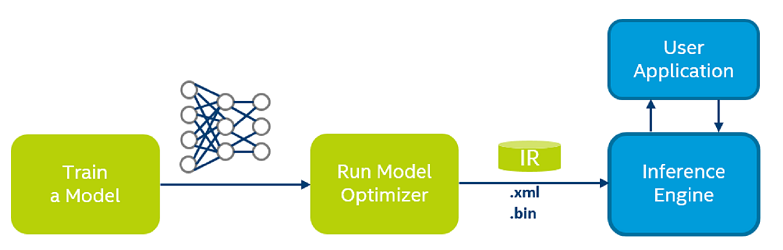
\includegraphics{./OpenVinoModelOptimizer}
	\caption{Workflow for deploying trained model onto NCS \autocite{ModelOptimizerDeveloper}}
	\label{fig:OpenVinoWorkflow}
\end{figure}


To pass the pruned and trained model to the Neural Compute stick OpenVino was used, it is a toolkit providing a high level \textbf{inference engine(Definition needed)} API, this facilitates the process of optimising the model for specialised hardware (in this case the NCS), and loading the optimised model into the NCS. 
OpenVino itself has a Benchmarking tool that we leverage to access to detailed latency and throughput metrics. A predefined set of images are selected and loaded into the NCS, the benchmarking application then runs 100 inference iterations network and returns the mean end-to-end latency (including loading images into the NCS memory), VPU processing latency (Inference latency), and throughput in FPS.

%! ---------------------------------------------------------------------------------------------------------------------------------
\subsection{Experiment setup}
\begin{itemize}
    \item Wrapper on Distiller, reading schedule \& paramaterise elements
    \item WandB implementation, defining parameters to optimise
    \item communication between producer \& consumer (redis - pub/sub)
    \item running benchmark and logging results
\end{itemize}

For the purpose of this experiment we chose to use the L1RankedStructureParameterPruner algorithm with both channel and filter pruning.

We conducted three experiments using the Resnet56 model trained on the CIFAR10 dataset. 
These three experiemnts each used a different target metric: Latency, Top1, and a hybrid metric (see section (TBD)).

\subsubsection{Schedules}
The following groups of weights were selected for pruning in the resnet56 model:

\begin{table}[H]
    \begin{tabular}{@{}|l|l|@{}}
        \toprule
        Lable & Weights \\
        \midrule
        filter\_pruner\_70 & module.layer1.0.conv1.weight,\\
        module.layer1.1.conv1.weight,\\
        module.layer1.2.conv1.weight,\\
        module.layer1.3.conv1.weight,\\
        module.layer1.4.conv1.weight,\\
        module.layer1.5.conv1.weight,\\
        module.layer1.6.conv1.weight,\\
        module.layer1.7.conv1.weight,\\
        module.layer1.8.conv1.weight
    \end{tabular}
\end{table}

\subsubsection{Latency Target Metric}
This experiment targeted pure inference latency, no information reguarding accuracy was encoded in the optimisation metric. 



\end{document}